\documentclass{report}
\usepackage[utf8]{inputenc}
\title{Resultados Tarea 4 Métodos Computacionales }
\author{Diego Felipe  Martinez Valencia}
\date{\today}
\usepackage{natbib}
\usepackage{parskip}
\usepackage{fancyhdr}
\usepackage{float}
\usepackage{graphicx}
\usepackage{subfigure}
\providecommand{\abs}[1]{\lvert#1\rvert}
\providecommand{\norm}[1]{\lVert#1\rVert}
\setlength{\textwidth}{170mm}
\setlength{\textheight}{230mm}
\setlength{\topmargin}{-20mm}
\setlength{\oddsidemargin}{-1mm}
\setlength{\evensidemargin}{30mm}
\usepackage{ragged2e}
\usepackage[usenames, dvipsnames]{color}
\usepackage[english]{babel}
\usepackage{color}
\begin{document}
\maketitle{}
\vspace*{-1cm}
\justify 
\section*{ODE}
En esta sección de muestran las gráficas de resultados del ejercicio de ecuaciones diferenciales ordinarias.
\begin{equation}
    \frac{d^{2}\vec{v}(t)}{dt^{2}}=-\vec{g}-c\frac{|\vec{v}(t)|^{2}}{m}\frac{\vec{v}(t)}{|\vec{v}(t)|}
\end{equation}
Inicialmente, para este caso se asignaron las siguientes condiciones iniciales:
\begin{equation}
    \vec{x}(t=0)=(0,0) \quad \vec{v}(t=0)=300(cos(\phi),sin(\phi))
\end{equation}
\subsection{Gráfica con ángulo de 45$^\circ$}
\begin{figure}[h]
    \centering
    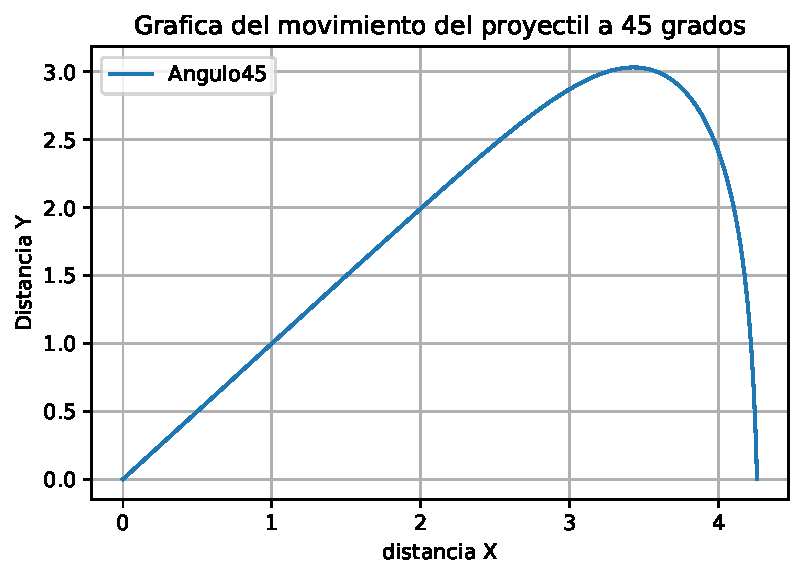
\includegraphics[scale = 0.5]{ODE_45grados.pdf}
    \caption{Gráfica de movimiento a 45 grados}
    \label{fig:my_label}
\end{figure}
De esta gráfica de la figura 1 es posible verificar que la distancia alcanzada es aproximadamente 7.95m. EN esta gráfica es posible ver un movimiento parabólico que sigue la partícula en movimiento, no está demás aclarar que este movimiento(como se vé en fisica 1) está dado por las fuerzas que actúan sobre la partícula. Aunque no se trate de meramente un problema de física 1, sino que el movimiento sea descrito como una ecuación diferencial ordinaria, la física detrás de este fenómeno es la misma.
\subsection{Gráfica con ángulos variables$^\circ$}
Con las mismas condiciones iniciales de la anterior figura:
\begin{figure}[h]
    \centering
    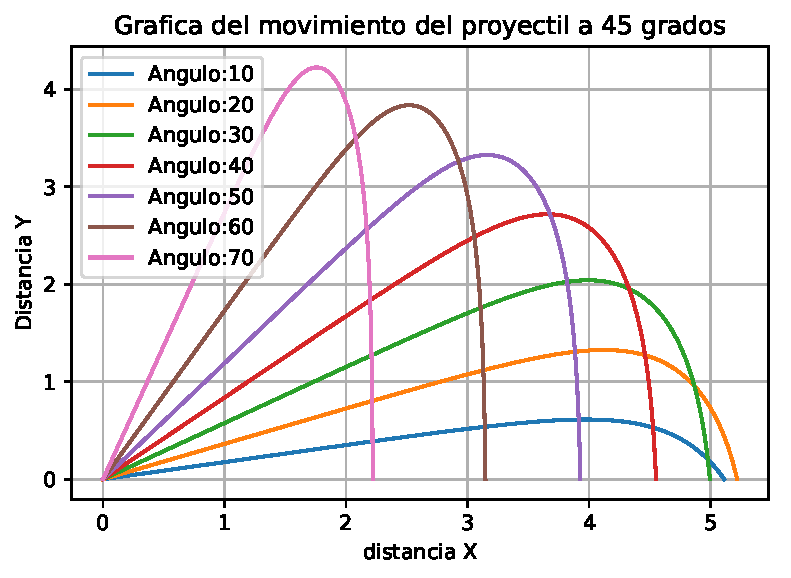
\includegraphics[scale = 0.5]{ODE_varicion_grados.pdf}
    \caption{Gráfica de movimiento a diferentes ángulos}
    \label{fig:my_label}
\end{figure}
De esta gráfica de la figura 2 es posible verificar que la distancia máxima alcanza se da cuando se tiene un ángulo de 20 grados.

\section*{PDE}
Comportamiento de la temperatura en una sección de una roca de calcita con una varilla cilíndrica incrustada perpendicularmente de diámetro 10cm. La ecuación que representa el sistema es la siguiente:

\begin{equation}
    \frac{dT(x,y)}{dt}=\nu\frac{d^{2}T(x,y)}{dx^{2}}+\nu\frac{d^{2}T(x,y)}{dy^{2}}
\end{equation}

La varilla posee una temperatura de 100$^{\circ}C$ constantes. Las condiciones iniciales de temperatura para la roca de calcita es de 10$^{\circ}C$ y las condiciones de frontera se dan para diferentes casos. Para cada caso, se realizo una simulación para un T = 1000*dt, con un dt = $ alpha*pow(dx,2)/v;$ donde v = $k_d/(Cp*rho)$. En cada uno, se realzaron 4 cuatro gráficas, que constatan la evolución de la temperatura en diferentes puntos del tiempo.

\subsection*{Condiciones de frontera fijas}
Se asignaron las condiciones de frontera a  10$^{\circ}C$ como se especifica en el enunciado. En este caso, se alcanzo un punto de estabilidad relativamente rápido comparado contra las gráficas de otras condiciones de frontera, pues en la gráfica c) se observa mínimo cambio con respecto a la gráfica en d).

\begin{figure}[H]
    \centering
    \subfigure[]{\label{PDE1_1}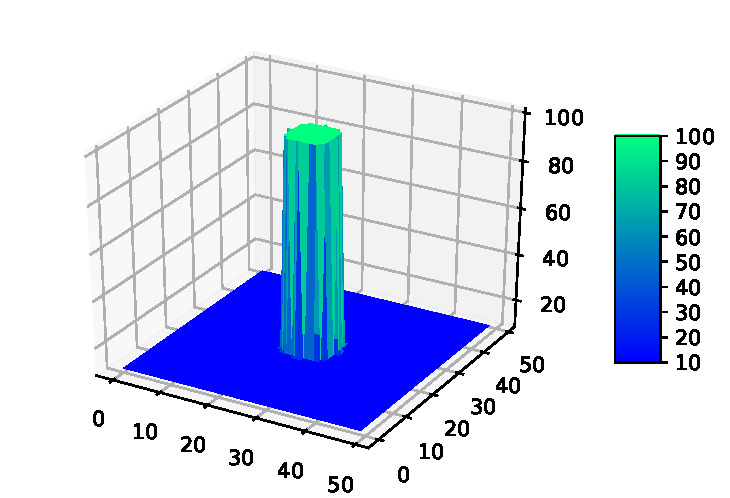
\includegraphics[scale = 0.6]{PDE_temp_10gc1.pdf}}
    \subfigure[]{\label{PDE1_2}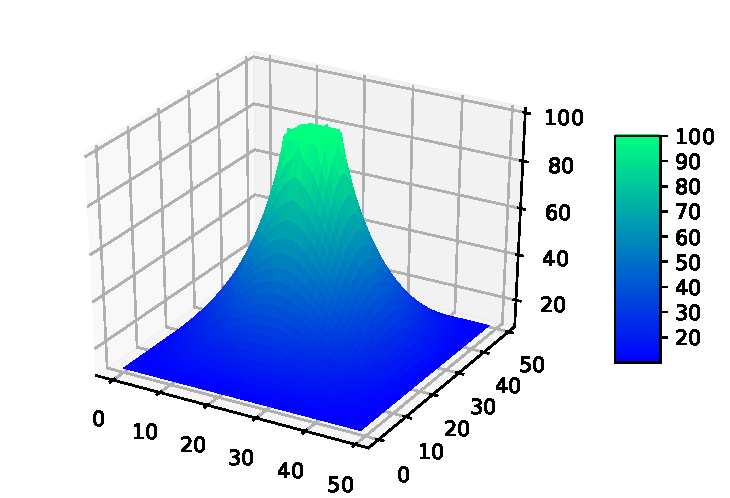
\includegraphics[scale = 0.6]{PDE_temp_10gc2.pdf}}
        \caption{Distribución de temperaturas para condiciones de frontera fijas a 10 grados centígrados a diferentes tiempos a) t=0, b) t=(2/3)t.}
    \label{fig:CondicionesFijasTemp}
\end{figure}
\begin{figure}[H]
    \centering 
    \subfigure[]{\label{PDE1_3}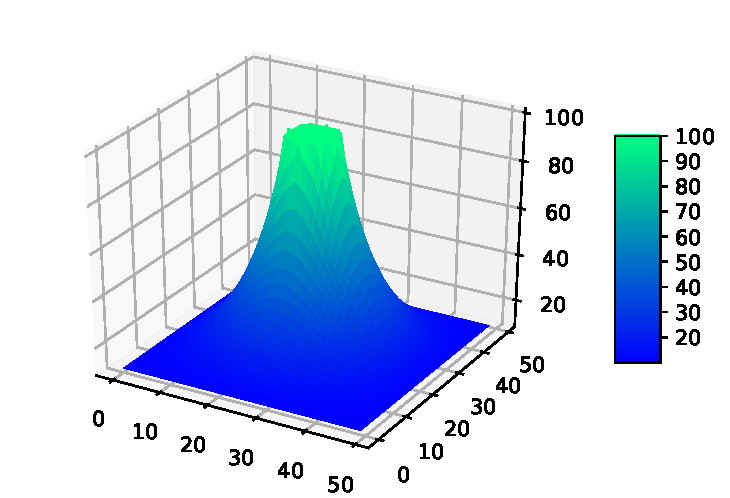
\includegraphics[scale = 0.6]{PDE_temp_10gc3.pdf}}
    \subfigure[]{\label{PDE1_4}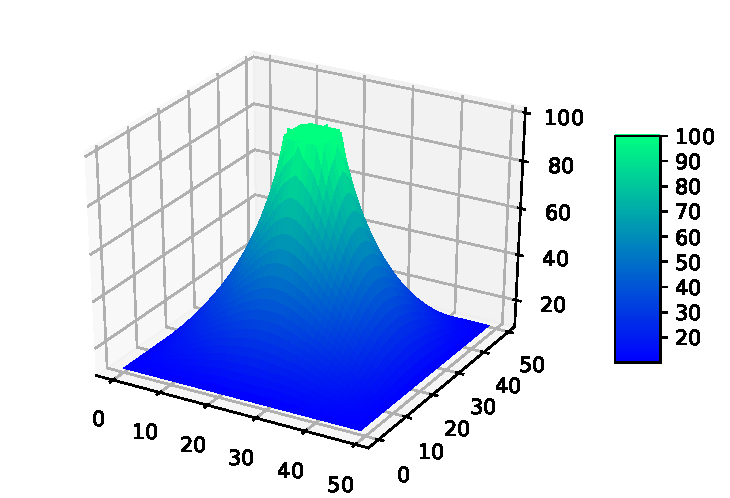
\includegraphics[scale = 0.6]{PDE_temp_10gc4.pdf}}
    \caption{Distribución de temperaturas para condiciones de frontera fijas a 10 grados centígrados a diferentes tiempos c) t=(1/3)t, d) t=t.}
    \label{fig:CondicionesFijasTemp}
\end{figure}


\subsection*{Condiciones de frontera abiertas}
En este caso se gráfica la solución con condiciones de frontera abiertas, aquí es posible observar que las fronteras empiezan gradualmente a aumentar su temperatura.En la ultima gráfica se puede ver como la temperatura aumenta mas gradualmente comportándose como una onda estacionaria.
\begin{figure}[H]
    \centering
    \subfigure[]{\label{PDE2_1}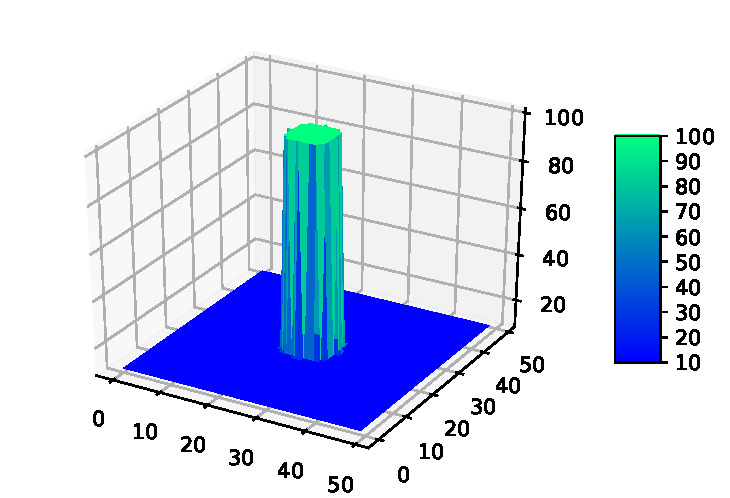
\includegraphics[scale = 0.6]{PDE_temp_Abiertas1.pdf}}
    \subfigure[]{\label{PDE2_2}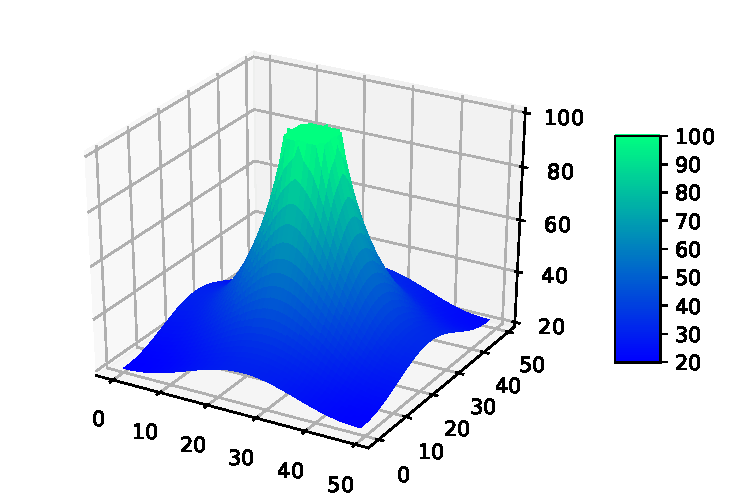
\includegraphics[scale = 0.6]{PDE_temp_Abiertas2.pdf}}
        \caption{Distribución de temperaturas para condiciones de frontera abiertas a diferentes tiempos a) t=0, b) t=(2/3)t.}
    \label{fig:Condicionesabieertas}
\end{figure}
\begin{figure}[H]
    \centering 
    \subfigure[]{\label{PDE2_3}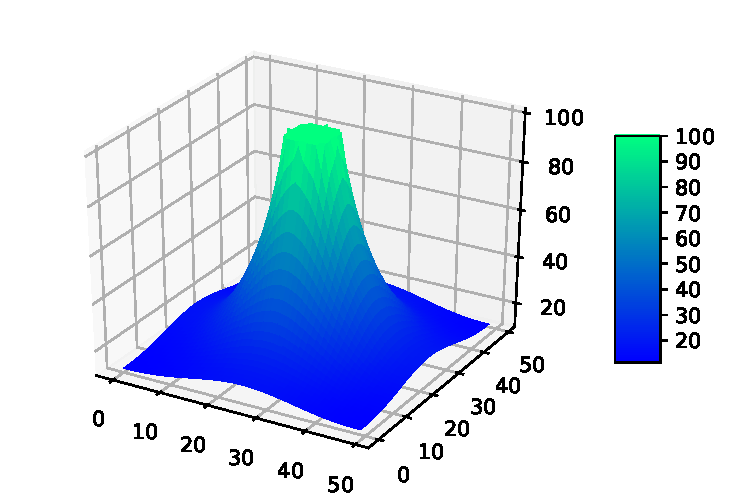
\includegraphics[scale = 0.6]{PDE_temp_Abiertas3.pdf}}
    \subfigure[]{\label{PDE2_4}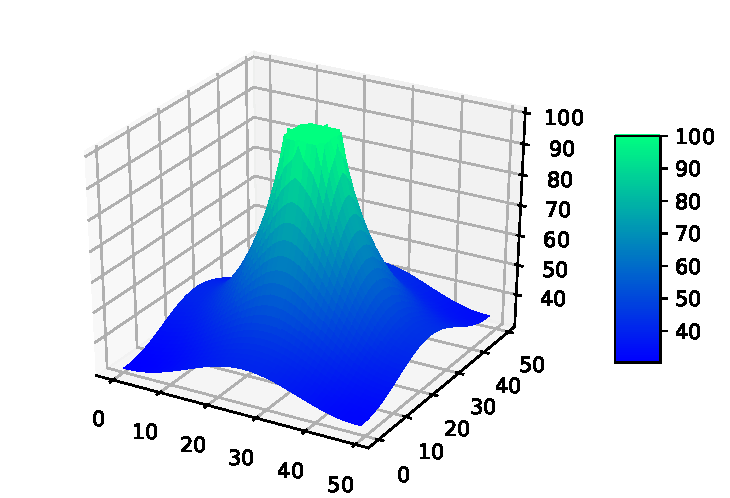
\includegraphics[scale = 0.6]{PDE_temp_Abiertas4.pdf}}
   \caption{Distribución de temperaturas para condiciones de frontera abiertas a diferentes tiempos a) t=0, b) t=(2/3)t.}
    \label{fig:Condicionesabiertas}
\end{figure}

\subsection*{Condiciones de frontera periódicas}
En este caso las condiciones de frontera se ajustan como periódicamente libres. Aquí es posible ver que la temperatura en las fronteras aumentan progresivamente. Aunque la última gráfica tiene una tendencia aumentar de manera mas lenta comportándose igualmente como una onda estacionaria.
\begin{figure}[H]
    \centering
    \subfigure[]{\label{PDE3_1}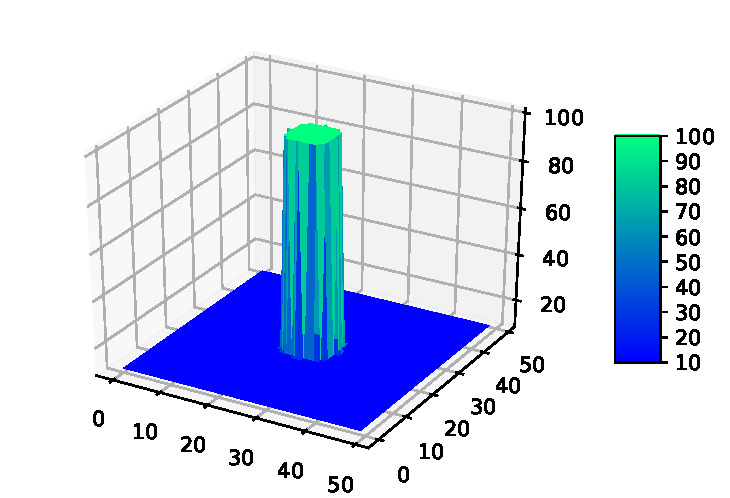
\includegraphics[scale = 0.6]{PDE_temp_periodicas1.pdf}}
    \subfigure[]{\label{PDE3_2}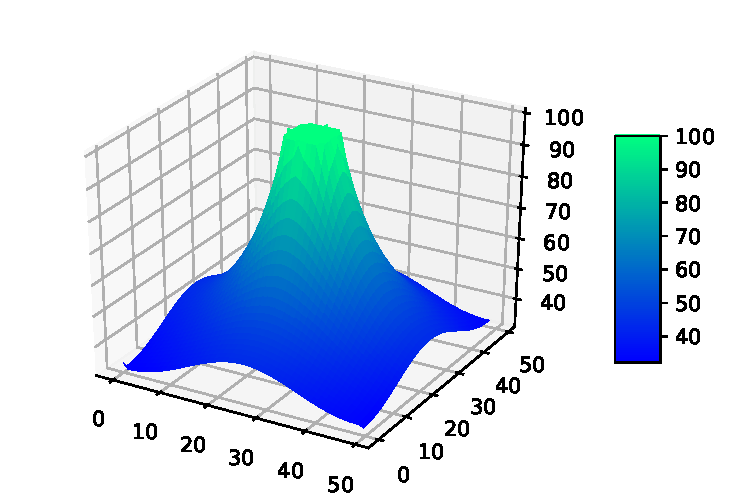
\includegraphics[scale = 0.6]{PDE_temp_Periodicas2.pdf}}
        \caption{Distribución de temperaturas para condiciones de frontera periódicas a diferentes tiempos a) t=0, b) t=(2/3)t.}
    \label{fig:Condicionesabieertas}
\end{figure}
\begin{figure}[H]
    \centering 
    \subfigure[]{\label{PDE3_3}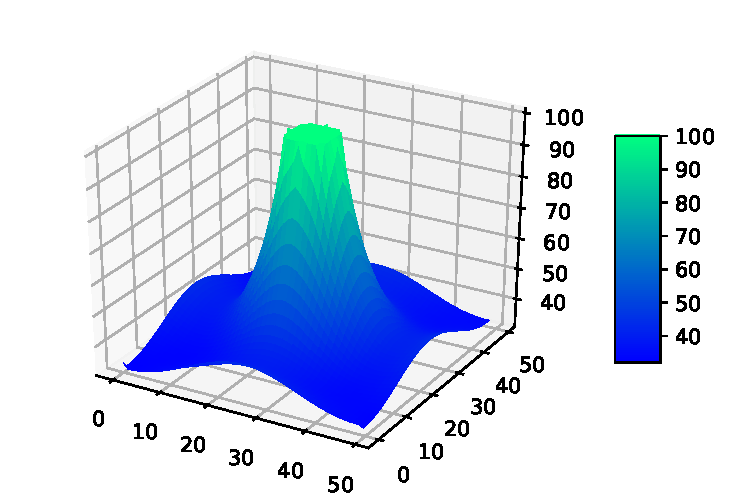
\includegraphics[scale = 0.6]{PDE_temp_Periodicas3.pdf}}
    \subfigure[]{\label{PDE3_4}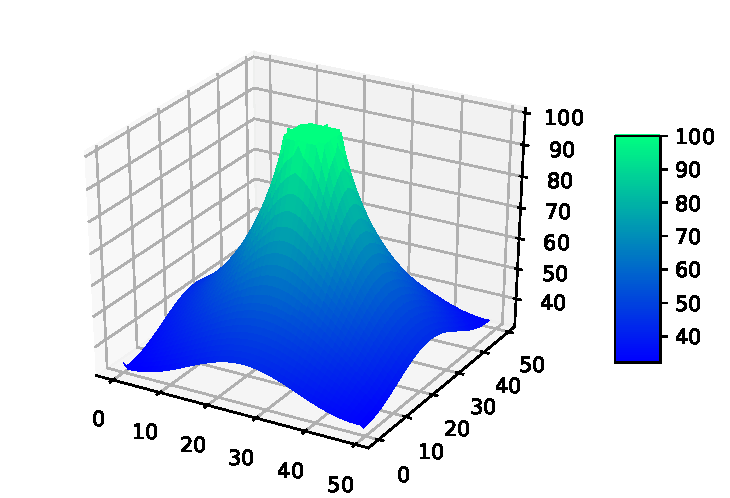
\includegraphics[scale = 0.6]{PDE_temp_Periodicas4.pdf}}
   \caption{Distribución de temperaturas para condiciones de frontera abiertas a diferentes tiempos a) t=0, b) t=(2/3)t.}
    \label{fig:Condicionesabiertas}
\end{figure}






\end{document}